\documentclass[journal,12pt,twocolumn]{IEEEtran}
\usepackage{setspace}
\usepackage{gensymb}
\usepackage{caption}
%\usepackage{multirow}
%\usepackage{multicolumn}
%\usepackage{subcaption}
%\doublespacing
\singlespacing
\usepackage{csvsimple}
\usepackage{amsmath}
\usepackage{multicol}
%\usepackage{enumerate}
\usepackage{amssymb}
%\usepackage{graphicx}
\usepackage{newfloat}
%\usepackage{syntax}
\usepackage{listings}
%\usepackage{iithtlc}
\usepackage{color}
\usepackage{siunitx}
\usepackage{tikz}
\usetikzlibrary{shapes,arrows}
\usepackage{circuitikz}



%\usepackage{graphicx}
%\usepackage{amssymb}
%\usepackage{relsize}
%\usepackage[cmex10]{amsmath}
%\usepackage{mathtools}
%\usepackage{amsthm}
%\interdisplaylinepenalty=2500
%\savesymbol{iint}
%\usepackage{txfonts}
%\restoresymbol{TXF}{iint}
%\usepackage{wasysym}
\usepackage{amsthm}
\usepackage{mathrsfs}
\usepackage{txfonts}
\usepackage{stfloats}
\usepackage{epstopdf}
\usepackage{cite}
\usepackage{cases}
\usepackage{mathtools}
\usepackage{caption}
\usepackage{enumerate}	
\usepackage{enumitem}
\usepackage{amsmath}
%\usepackage{xtab}
\usepackage{longtable}
\usepackage{multirow}
%\usepackage{algorithm}
%\usepackage{algpseudocode}
\usepackage{enumitem}
\usepackage{mathtools}
\usepackage{hyperref}
%\usepackage[framemethod=tikz]{mdframed}
\usepackage{listings}
    %\usepackage[latin1]{inputenc}                                 %%
    \usepackage{color}                                            %%
    \usepackage{array}                                            %%
    \usepackage{longtable}                                        %%
    \usepackage{calc}                                             %%
    \usepackage{multirow}                                         %%
    \usepackage{hhline}                                           %%
    \usepackage{ifthen}                                           %%
  %optionally (for landscape tables embedded in another document): %%
    \usepackage{lscape}     


\usepackage{url}
\def\UrlBreaks{\do\/\do-}


%\usepackage{stmaryrd}


%\usepackage{wasysym}
%\newcounter{MYtempeqncnt}
\DeclareMathOperator*{\Res}{Res}
%\renewcommand{\baselinestretch}{2}
\renewcommand\thesection{\arabic{section}}
\renewcommand\thesubsection{\thesection.\arabic{subsection}}
\renewcommand\thesubsubsection{\thesubsection.\arabic{subsubsection}}

\renewcommand\thesectiondis{\arabic{section}}
\renewcommand\thesubsectiondis{\thesectiondis.\arabic{subsection}}
\renewcommand\thesubsubsectiondis{\thesubsectiondis.\arabic{subsubsection}}

% correct bad hyphenation here
\hyphenation{op-tical net-works semi-conduc-tor}

%\lstset{
%language=C,
%frame=single, 
%breaklines=true
%}

%\lstset{
	%%basicstyle=\small\ttfamily\bfseries,
	%%numberstyle=\small\ttfamily,
	%language=Octave,
	%backgroundcolor=\color{white},
	%%frame=single,
	%%keywordstyle=\bfseries,
	%%breaklines=true,
	%%showstringspaces=false,
	%%xleftmargin=-10mm,
	%%aboveskip=-1mm,
	%%belowskip=0mm
%}

%\surroundwithmdframed[width=\columnwidth]{lstlisting}
\def\inputGnumericTable{}                                 %%
\lstset{
%language=C,
frame=single, 
breaklines=true,
columns=fullflexible
}
 

\begin{document}
%
\tikzstyle{block} = [rectangle, draw,
    text width=3em, text centered, minimum height=3em]
\tikzstyle{sum} = [draw, circle, node distance=3cm]
\tikzstyle{input} = [coordinate]
\tikzstyle{output} = [coordinate]
\tikzstyle{pinstyle} = [pin edge={to-,thin,black}]

\theoremstyle{definition}
\newtheorem{theorem}{Theorem}[section]
\newtheorem{problem}{Problem}
\newtheorem{proposition}{Proposition}[section]
\newtheorem{lemma}{Lemma}[section]
\newtheorem{corollary}[theorem]{Corollary}
\newtheorem{example}{Example}[section]
\newtheorem{definition}{Definition}[section]
%\newtheorem{algorithm}{Algorithm}[section]
%\newtheorem{cor}{Corollary}
\newcommand{\BEQA}{\begin{eqnarray}}
\newcommand{\EEQA}{\end{eqnarray}}
\newcommand{\define}{\stackrel{\triangle}{=}}
\bibliographystyle{IEEEtran}
%\bibliographystyle{ieeetr}
\providecommand{\nCr}[2]{\,^{#1}C_{#2}} % nCr
\providecommand{\nPr}[2]{\,^{#1}P_{#2}} % nPr
\providecommand{\mbf}{\mathbf}
\providecommand{\pr}[1]{\ensuremath{\Pr\left(#1\right)}}
\providecommand{\qfunc}[1]{\ensuremath{Q\left(#1\right)}}
\providecommand{\sbrak}[1]{\ensuremath{{}\left[#1\right]}}
\providecommand{\lsbrak}[1]{\ensuremath{{}\left[#1\right.}}
\providecommand{\rsbrak}[1]{\ensuremath{{}\left.#1\right]}}
\providecommand{\brak}[1]{\ensuremath{\left(#1\right)}}
\providecommand{\lbrak}[1]{\ensuremath{\left(#1\right.}}
\providecommand{\rbrak}[1]{\ensuremath{\left.#1\right)}}
\providecommand{\cbrak}[1]{\ensuremath{\left\{#1\right\}}}
\providecommand{\lcbrak}[1]{\ensuremath{\left\{#1\right.}}
\providecommand{\rcbrak}[1]{\ensuremath{\left.#1\right\}}}
\theoremstyle{remark}
\newtheorem{rem}{Remark}
\newcommand{\sgn}{\mathop{\mathrm{sgn}}}
%\providecommand{\abs}[1]{\left\vert#1\right\vert}
\providecommand{\res}[1]{\Res\displaylimits_{#1}} 
\providecommand{\norm}[1]{\lVert#1\rVert}
\providecommand{\mtx}[1]{\mathbf{#1}}
%\providecommand{\mean}[1]{E\left[ #1 \right]}
\providecommand{\fourier}{\overset{\mathcal{F}}{ \rightleftharpoons}}
%\providecommand{\hilbert}{\overset{\mathcal{H}}{ \rightleftharpoons}}
\providecommand{\system}{\overset{\mathcal{H}}{ \longleftrightarrow}}
	%\newcommand{\solution}[2]{\textbf{Solution:}{#1}}
\newcommand{\solution}{\noindent \textbf{Solution: }}
\newcommand{\myvec}[1]{\ensuremath{\begin{pmatrix}#1\end{pmatrix}}}
\providecommand{\dec}[2]{\ensuremath{\overset{#1}{\underset{#2}{\gtrless}}}}
\DeclarePairedDelimiter{\ceil}{\lceil}{\rceil}
%\numberwithin{equation}{section}
%\numberwithin{problem}{subsection}
%\numberwithin{definition}{subsection}
\makeatletter
\@addtoreset{figure}{section}
\makeatother
\let\StandardTheFigure\thefigure
%\renewcommand{\thefigure}{\theproblem.\arabic{figure}}
\renewcommand{\thefigure}{\thesection}
%\numberwithin{figure}{subsection}
%\numberwithin{equation}{subsection}
%\numberwithin{equation}{section}
%\numberwithin{equation}{problem}
%\numberwithin{problem}{subsection}
\numberwithin{problem}{section}
%%\numberwithin{definition}{subsection}
%\makeatletter
%\@addtoreset{figure}{problem}
%\makeatother
\makeatletter
\@addtoreset{table}{section}
\makeatother
\let\StandardTheFigure\thefigure
\let\StandardTheTable\thetable
\let\vec\mathbf
%%\renewcommand{\thefigure}{\theproblem.\arabic{figure}}
%\renewcommand{\thefigure}{\theproblem}
%%\numberwithin{figure}{section}
%%\numberwithin{figure}{subsection}
\def\putbox#1#2#3{\makebox[0in][l]{\makebox[#1][l]{}\raisebox{\baselineskip}[0in][0in]{\raisebox{#2}[0in][0in]{#3}}}}
     \def\rightbox#1{\makebox[0in][r]{#1}}
     \def\centbox#1{\makebox[0in]{#1}}
     \def\topbox#1{\raisebox{-\baselineskip}[0in][0in]{#1}}
     \def\midbox#1{\raisebox{-0.5\baselineskip}[0in][0in]{#1}}
\vspace{3cm}
\title{ 
%	\logo{
Internal Circuit Analysis OF LM7809 Voltage Regulator
%	}
}
\author{ Lakshit Singla and Hema Varshita $^{*}$% <-this % stops a space
	\thanks{*The author is with the Department
		of Electrical Engineering, Indian Institute of Technology, Hyderabad
		502285 India e-mail:  gadepall@iith.ac.in. All solutions in this manual is released under GNU 
GPL.  Free and open source.}
	
}
\maketitle
\tableofcontents
\bigskip
\renewcommand{\thefigure}{\theenumi}
\renewcommand{\thetable}{\theenumi}
\begin{abstract}
This manual provides the IC analysis for the LM7809 voltage regulator. 
\end{abstract}
\section{Equivalent Circuit of LM7809}
%\begin{enumerate}[label=\arabic*]
\begin{enumerate}[label=\thesection.\arabic*,ref=\thesection.\theenumi]
\numberwithin{equation}{enumi}
\item abcd
%\begin{figure}[!ht]
%\centering
%\caption{}
%\label{fig:1}
%\end{figure}
\begin{figure}[!ht]
%\begin{center}
\centering	
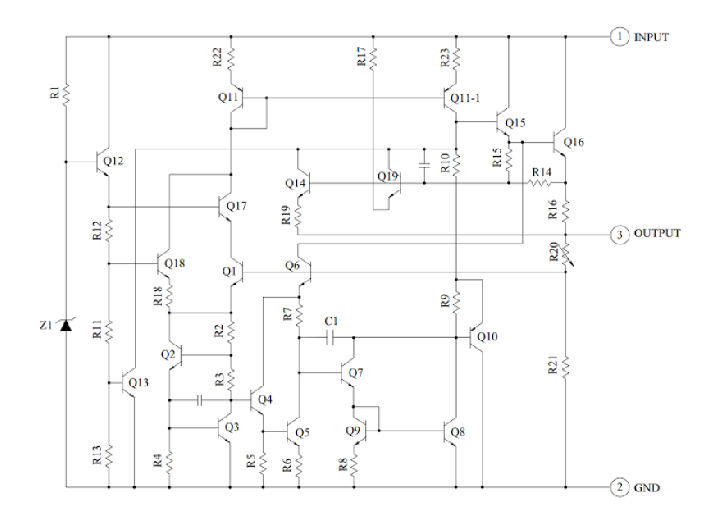
\includegraphics[width=\columnwidth]{./figs/Mainfig.eps}
%\vspace*{-10cm}
%\end{center}
\caption{LM7809 Regulator}
\label{fig:orig}	
\end{figure}
\end{enumerate}

\section{ Components of the regulator:}
\begin{enumerate}[label=\thesection.\arabic*,ref=\thesection.\theenumi]
\numberwithin{equation}{enumi}
\item Analyse and Divide the circuit based on it's functionality\\
\solution
\begin{figure}[!ht]
\centering	
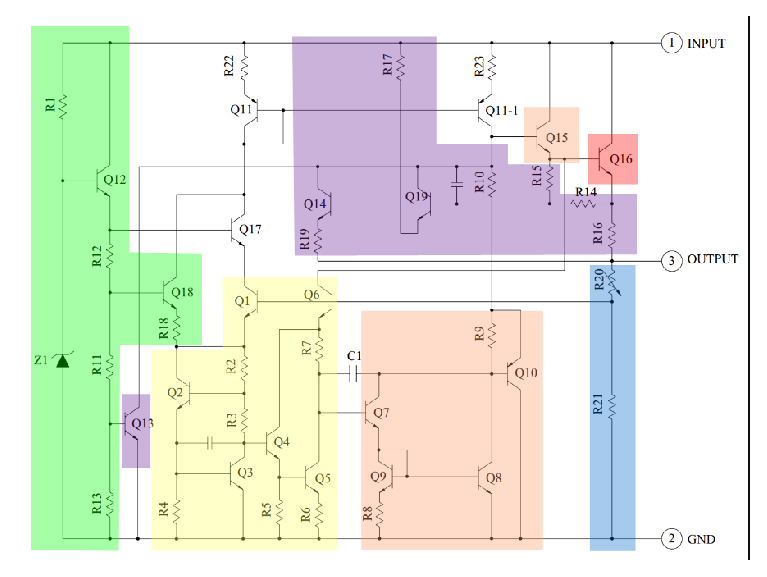
\includegraphics[width=\columnwidth]{./figs/Colorfig.eps}
\caption{LM7809 Regulator}
\label{fig:2}
\end{figure}
The internal circuit predominantly consists of 1 zener diode, 1 cap,19 transistors and 23 resistors
%\hskip 

\item State the function of each colour coded circuit in Fig 2.1\\
\solution
Based on the functionality, the internal circuit is divided into 6 parts namely: \\
 1. Band gap Reference \\
 2. Startup\\
 3. Protection \\
 4. Error Amplifier\\
 5. Voltage Divider \\
 6. Output
\end{enumerate}

\section{Band gap Reference}
\begin{enumerate}[label=\thesection.\arabic*,ref=\thesection.\theenumi]
\numberwithin{equation}{enumi}
\item The circuit coded by yellow colour perdorms band gap reference operations
\item  What is the input of Band gap reference part of the circuit?\\
\solution
The circuit takes scaled output voltage as input at Q1 and Q6 transistor. 
\item  What is the output of the circuit?\\
\solution 
It provides an error signal as output and sends it to Q7 as an error signal indicating if the voltage is too high or too low.
\item What is the importance of the circuit?\\
\solution
It stabilises the output voltage and provides a stable and accurate reference, even as the chip's temperature changes.
\end{enumerate}

\section{Startup}
\begin{enumerate}[label=\thesection.\arabic*,ref=\thesection.\theenumi]
\numberwithin{equation}{enumi}
\item The circuit coded by green colour denotes the part of circuit that provides Startup to the circuit
\item Band gap circuits usually have two stable voltages - the
desired voltage and 0 volts.
\item To keep the band gap from getting stuck at 0 volts, a startup
circuit will ”push” the band gap away from 0 volts so it will
settle at the desired voltage.
\end {enumerate}

\section{Protection}
\begin{enumerate}[label=\thesection.\arabic*,ref=\thesection.\theenumi]
\numberwithin{equation}{enumi}
\item The circuit coded by purple colour denotes the part of circuit that provides protection to the circuit
\item Which transistors in the circuit provide protection?\\
\solution
(Q13) - Protection against Overheating\\
(Q19) - Protection against excessive input voltage\\
(Q14) - Protection against excessive output current
\item How does the circuit ensure Protection?\\
\solution
If there is a fault, these circuits reduce the output current or
shut down the regulator, protecting it from damage.

\section{Error amplifier}
\begin{enumerate}[label=\thesection.\arabic*,ref=\thesection.\theenumi]
\numberwithin{equation}{enumi}
\item The circuit coded by pink colour 
\item The error signal from the band gap reference is amplified by
the error amplifier.
\item Why do we need to amplify the error signal?\\
\solution
The error signal needs to be amplified so it can control the output voltage through the Q15 transistor
\end{enumerate}

\section{Voltage Divider}
\begin{enumerate}[label=\thesection.\arabic*,ref=\thesection.\theenumi]
\numberwithin{equation}{enumi}
\item Denoted by blue color code
\item The voltage divider scales down the voltage on the output pin
for use by the band gap reference
\item For any general LM78XX regulator, a simple change to the position of the variable contact increases the resistance of R20 and thus
the output voltage of the chip.
\end{enumerate}


\section{Output}
\begin{enumerate}[label=\thesection.\arabic*,ref=\thesection.\theenumi]
\numberwithin{equation}{enumi}
\item Q16 controls the current between the input and output, and thus controls the output voltage.

\end{enumerate}

\end{enumerate}
\end{document}















